\documentclass{article}

\usepackage{listings}
\usepackage{graphicx}
\usepackage{cite}

\title{BRS Readout Description}
\author{M.P.Ross}
\begin{document}
\maketitle
\section{Introduction}
This document describes the ``BRSReadout'' software which was developed by the E{\"o}t-Wash group as the main readout of the Beam Rotation Sensor (BRS). The BRS's angular readout is achieved using a multi-slit autocollimator refined from the device described in \cite{autoCol}. The goal of the software is to turn line camera images into an number of angular readout channels while also giving the user an interface to view the camera images, plot the angular data, record data to disk, and monitor performance.
\section{Image Analysis}

\section{Signal Processing}
\section{User Interface}

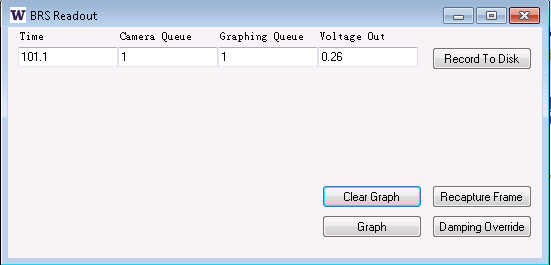
\includegraphics[width=\textwidth]{BRSReadoutScreen.png}\\
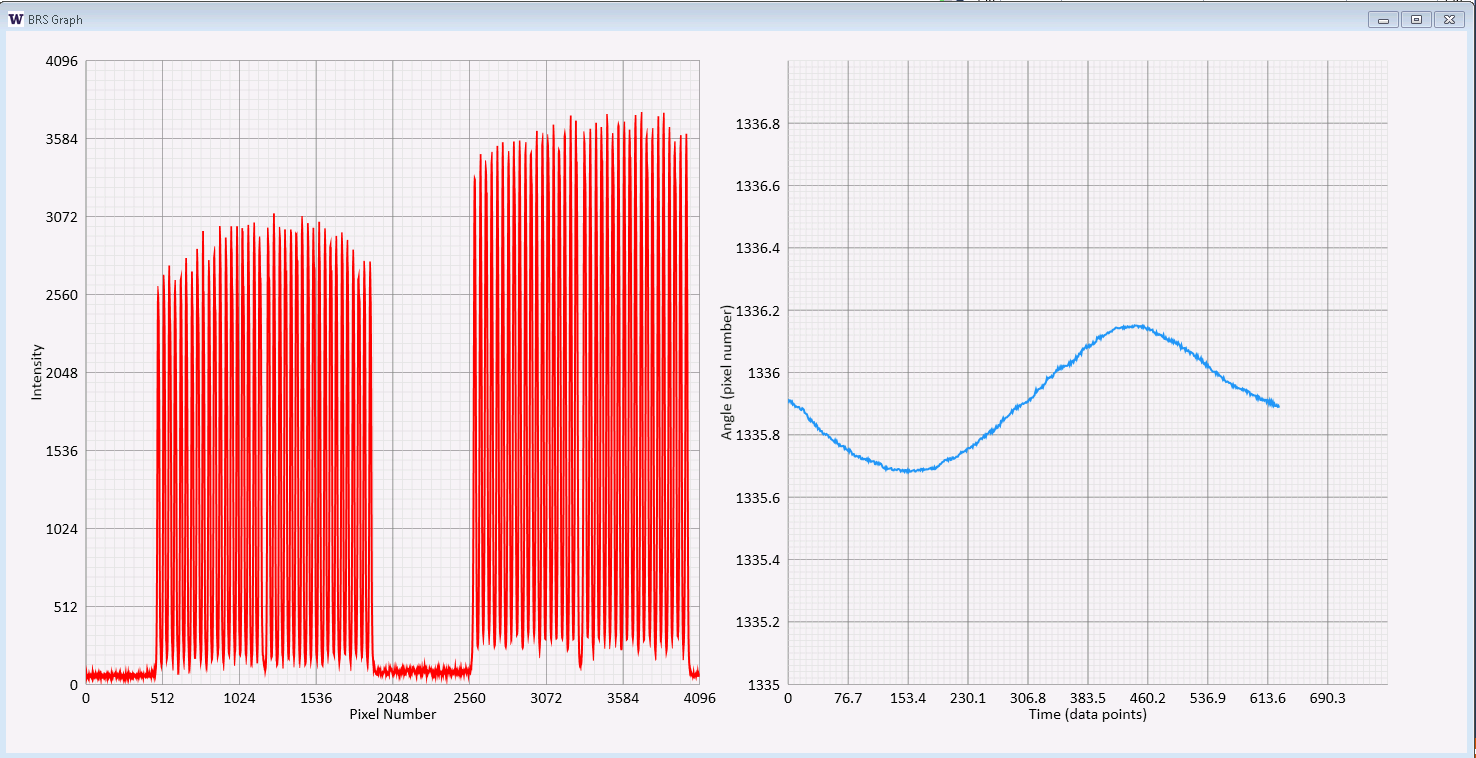
\includegraphics[width=\textwidth]{BRSReadoutScreenGraph.png}

\bibliographystyle{plain}
\bibliography{ReadoutDescription}{}
\end{document}